% Copyright (c)  2005-2010 EDF-EADS-PHIMECA.
% Permission is granted to copy, distribute and/or modify this document
% under the terms of the GNU Free Documentation License, Version 1.2
% or any later version published by the Free Software Foundation;
% with no Invariant Sections, no Front-Cover Texts, and no Back-Cover
% Texts.  A copy of the license is included in the section entitled "GNU
% Free Documentation License".
\renewcommand{\filename}{docUC_StochProc_RandomWalk.tex}
\renewcommand{\filetitle}{UC : Manipulation of a Random Walk}

% \HeaderNNIILevel
 \HeaderIILevel
%\HeaderIIILevel

\label{processWN}

\index{Stochastic Process!Random Walk}


This section details first how to create and manipulate a random walk.\\

A random walk $(\underline{X}_n(\omega))_{ n\geq 0}$ is a discrete time stochastic process such that:
\begin{eqnarray}
  \vect{X}_0(\omega) & = & \vect{x}_0 \\
  \forall n>0,\:\vect{X}_n(\omega) & = & \vect{X}_{n-1}(\omega) + \vect{\epsilon}_n(\omega)
\end{eqnarray}
where $\vect{x}_0$ is a given point in $\mathbb{R}^d$ and $\vect{\epsilon}_n(\omega)$ is a $d$ dimensional white noise distributed according to a given distribution $\mathcal{D}$. 

A random walk is a discrete time stochastic process with independent, identically distributed increments (or steps) as $\forall n>0,\:\vect{X}_n-\vect{X}_{n-1}=\vect{\epsilon}_n$. The given distribution $\mathcal{D}$ is the common distribution of these steps, with no restriction on this distribution. It is thus possible to define discrete state random walks such as walks over a lattice by using a discrete distribution (such as the {\itshape UserDefined} distribution or the other discrete distributions defined in Open TURNS), or a continuous state random walk using e.g. a Normal distribution.

 Open TURNS proposes to model it through the object \emph{RandomWalk} defined thanks to :
\begin{itemize}
\item an origin;
\item a distribution;
\item a time grid.
\end{itemize}


The $RandomWalk$ object inherits from $Process$ object. Thus, it is possible to get its marginal process, its time grid, its dimension and to get several realization at a time of the process.\\

Details on each object may be found in the User Manual  (\href{OpenTURNS_UserManual_TUI.pdf}{see User Manual - Stochastic Process}).\\

\requirements{
  \begin{description}
  \item[$\bullet$] a numerical point : {\itshape $myOrigin$}
  \item[type:] NumericalPoint
  \end{description}

  \begin{description}
  \item[$\bullet$] a distribution : {\itshape $myDistribution$}
  \item[type:]  Distribution
  \end{description}

  \begin{description}
  \item[$\bullet$] a time grid : {\itshape $myTimeGrid$}
  \item[type:]  RegularGrid
  \end{description}

}
{
  \begin{description}
  \item[$\bullet$] a random walk {\itshape myRandomWalk}
  \item[type:]  RandomWalk
  \end{description}
}

\textspace\\
Python script for this UseCase :

\begin{lstlisting}

  # Creation of a random walk
  # From an origin, a distribution and a time grid
  myRandomWalk = RandomWalk(myOrigin, myDistribution, myTimeGrid)

  # Creation of a random walk
  # using an origin, a distribution and the default RegularGrid 
  # care! This RegularGrid begins at time t = 0
  myRandomWalk = RandomWalk(myOrigin, myDistribution)

  # Get a realization of the process
  realization = myRandomWalk.getRealization()

  # Get a sample of N realizations of the process
  sample = myRandomWalk.getSample(N)

  # Get the i-th marginal of the process
  myMarginalRandomWalk = myRandomWalk.getMarginalProcess(i)

  # Get the marginal of index in indices of the process   
  myMarginalRandomWalk = myRandomWalk.getMarginalProcess(indices)

  # Get the distribution of the Random Walk
  myRandomWalkDistribution = myRandomWalk.getDistribution()

  # Set a new distribution for the Random Walk
  myRandomWalkDistribution.setDistribution(newDistribution)
 
  # Print the marginal of index i wrt the time
  myGraph = sample.drawMarginal(i)

  # Print n realizations of both marginals $i$ anf $j$ in the phase space Xi versus Xj
  # from a process of dimension d 
  sample = myRandomWalk.getSample(n)
  myGraph = Graph('2D Random Walk - Marginals i and j', 'Xi', 'Xj', True)
  # define the colors used for the n trajectories
  pal=Drawable.GetValidColors()
  for k in range(n) : 
    # get the values (of dimension d) of the time series of index k
    values = sample[k].getNumericalSample()
    # get the values of marginals i anj
    marginalValues = values.getMarginal(Indices(i,j))
    # add the trajectory into the graph with color pal[k]
    myGraph.add(Curve(marginalValues, pal[k], 'solid'))
  \end{lstlisting}

\textspace\\
Figures (\ref{randomwalk1D_Discrete}) and (\ref{randomwalk1D_Continuous}) illustrate realizations of a 1D random walk where the distribution $\mathcal{D}$ is respectively :
\begin{itemize}
  \item discrete :  the support is the two points $\{-1, 10\}$ with respective weights $0.9$ and $0.1$,
  \item continuous : the Normal distribution $\mathcal{N}(0,1)$.
\end{itemize}



\begin{figure}[H]
  \begin{minipage}{9cm}
    \begin{center}
      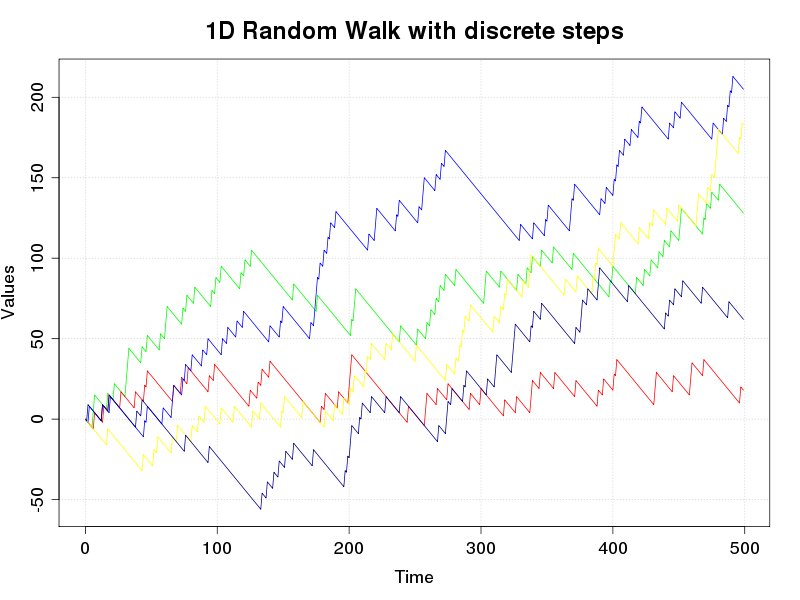
\includegraphics[width=7cm]{randomwalk1D_discrete.png}
      \caption{Realizations of a random walk with the discrete distribution : $P(-1) = 0.9, P(10)=0.1$.}
      \label{randomwalk1D_Discrete}
    \end{center}
  \end{minipage}
  \hfill
  \begin{minipage}{9cm}
    \begin{center}
      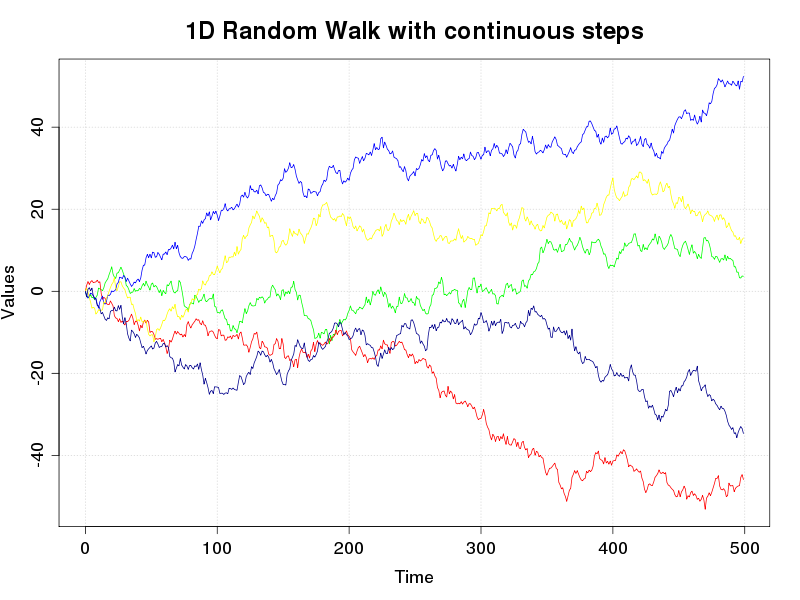
\includegraphics[width=7cm]{randomwalk1D_continuous.png}
      \caption{Realizations of a random walk with distribution $\mathcal{N}(0,1)$.}
      \label{randomwalk1D_Continuous}
    \end{center}
  \end{minipage}
\end{figure}

Figures (\ref{randomwalk2D_Discrete}) and (\ref{randomwalk2D_Continuous}) illustrate realizations of a 2D random walk where the distribution $\mathcal{D}$ is respectively :
\begin{itemize}
  \item discrete :  the support is the two points $\{-1, 10\}$ with respective weights $0.9$ and $0.1$,
  \item continuous : the 2D Normal distribution $\mathcal{N}(\vect{0},\mat{1})$.
\end{itemize}
The realizations are  presented in the phase space $X_1$ versus $X_2$.


\begin{figure}[H]
  \begin{minipage}{9cm}
    \begin{center}
      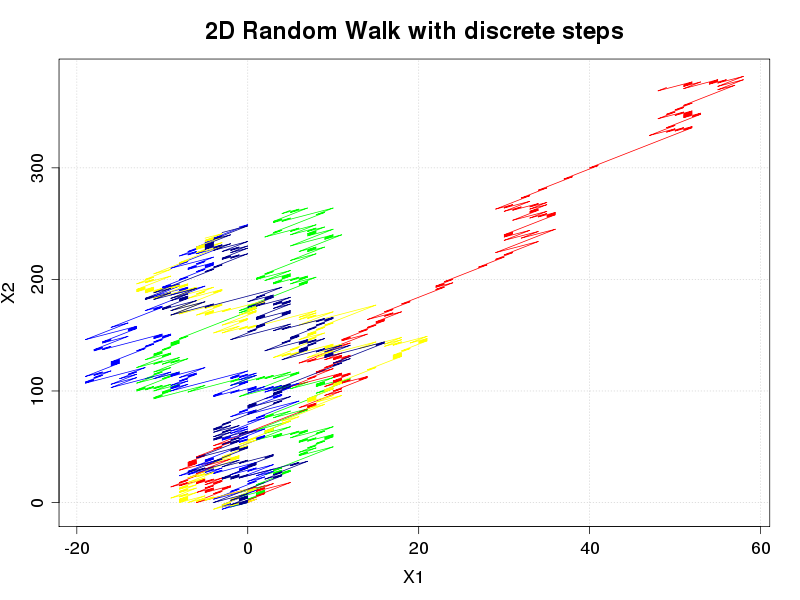
\includegraphics[width=7cm]{randomwalk2D_discrete.png}
      \caption{Realizations of a random walk with the uniform discrete distribution over the points $(-1, -2)$ and $(1,3)$.}
      \label{randomwalk2D_Discrete}
    \end{center}
  \end{minipage}
  \hfill
  \begin{minipage}{9cm}
    \begin{center}
      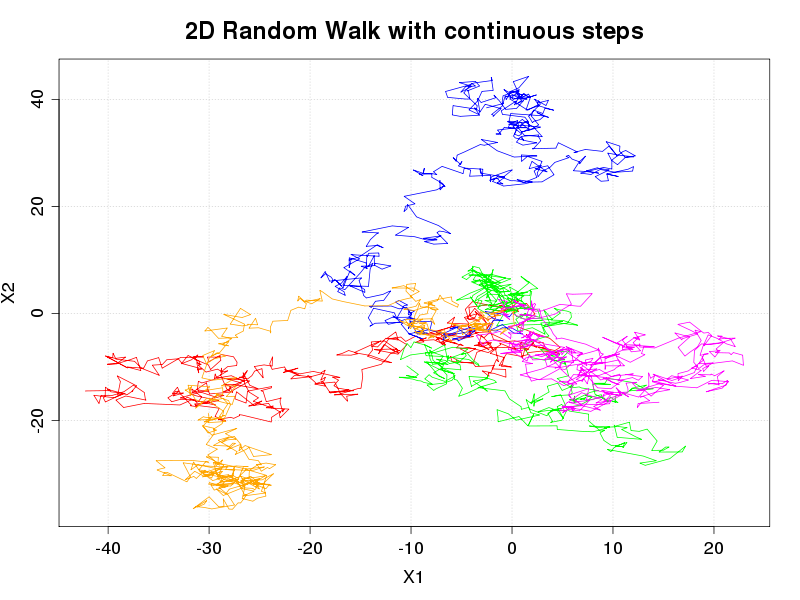
\includegraphics[width=7cm]{randomwalk2D_continuous.png}
      \caption{5 realizations of a random walk with distribution $\mathcal{N}(\vect{0},\mat{I})$}
      \label{randomwalk2D_Continuous}
    \end{center}
  \end{minipage}
\end{figure}
